% !TeX spellcheck = en_GB
\section{Haukeliseter site}\label{sec:dim:site}
% and some more
%\subsection{Measurement site and climate}
%%% images measurement site %%%%%%%%%%%%%%%%%%%%%%%%%%%%%%%%%%%%%
% !TeX spellcheck = en_GB
\begin{figure}[!b]
	\centering
    \begin{subfigure}[b]{0.55\textwidth}
    	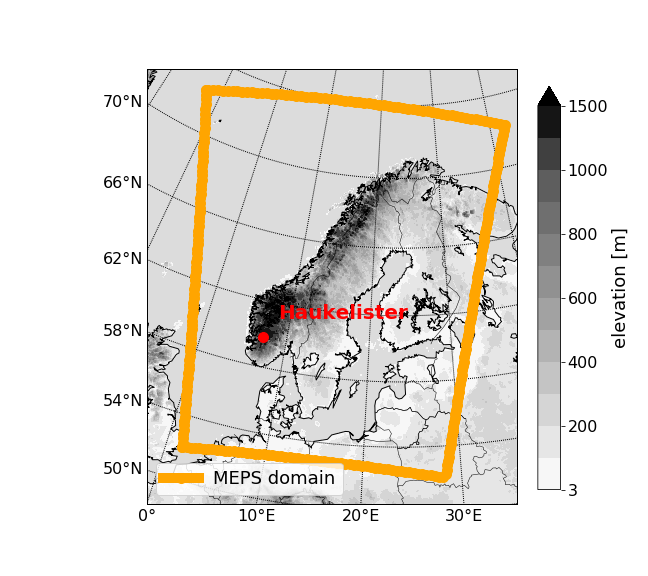
\includegraphics[trim={4.cm 1.8cm 0cm 2.2cm},clip,width=\textwidth]{./fig_Norway/Norway_elevation}
        \caption{}\label{fig:site:Norway}
    \end{subfigure}
    \begin{subfigure}[b]{0.44\columnwidth}
        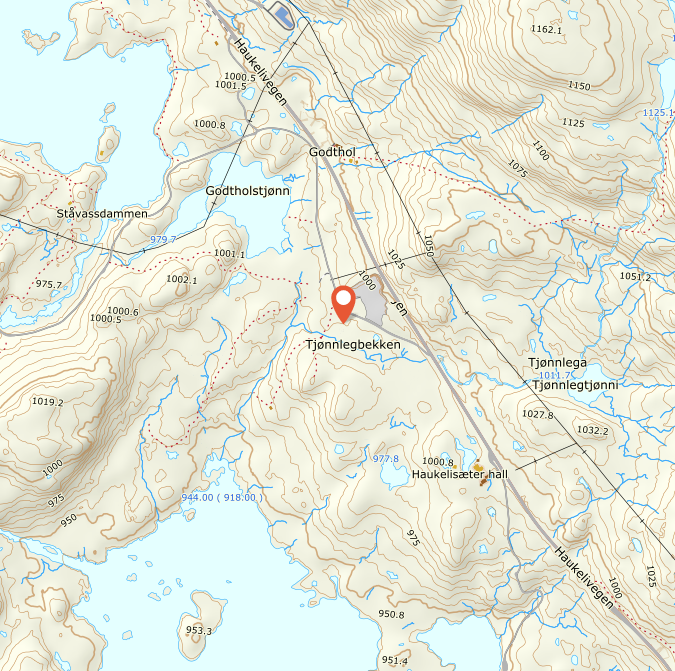
\includegraphics[trim={.3cm 2.2cm 1.8cm 2.4cm},clip,width=\textwidth]{./fig_Norway/Haukeli_site}
        \caption{}\label{fig:site:kartverket}
      \end{subfigure}
	\caption{\protect\subref{fig:site:Norway}: Elevation map of Northern Europe, data taken from \citet{noaa_etopo1_nodate}. \protect\subref{fig:site:kartverket}: Topographic map of the measurement site Haukeliseter \citep{kartverket_norgeskart_2018}.}\label{fig:site}
\end{figure} 
% \begin{figure}[t]
% 	\centering
% 	\begin{subfigure}[b]{0.49\textwidth}
% 		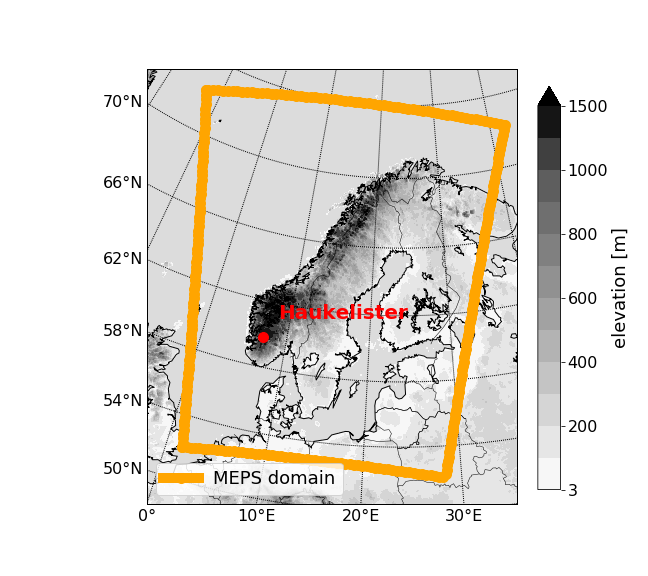
\includegraphics[trim={5.cm 1.8cm 5.8cm 2.3cm},clip,
% 		width=\textwidth]{./fig_Norway/Norway_MEPS}
% 		\caption{}\label{fig:site:Norway}
% 	\end{subfigure}
% 	%%%%% zoomed in map
% 	\begin{subfigure}[b]{0.49\textwidth}
% 		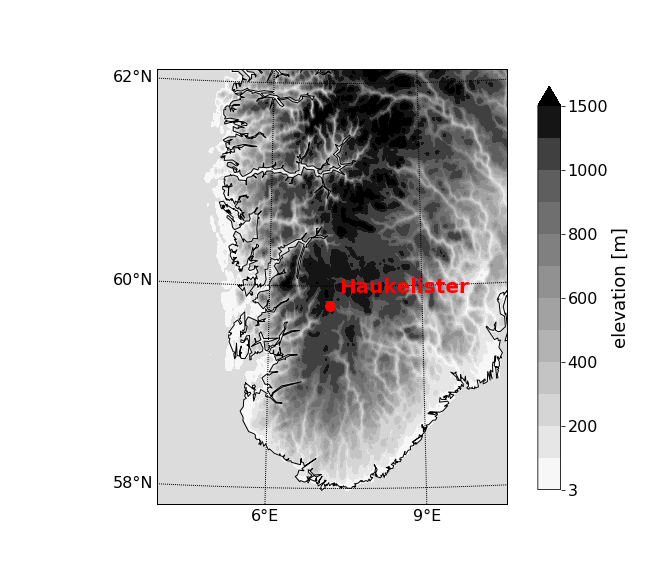
\includegraphics[trim={2.cm 1.8cm .65cm 2.3cm},clip,
% 		width=\textwidth]{./fig_Norway/South_Norway}
% 		\caption{}\label{fig:site:Nzoom}
% 	\end{subfigure}
% 	%%%%% zoomed in kartverketmap
% 	\begin{subfigure}[b]{0.32\textwidth}
% 		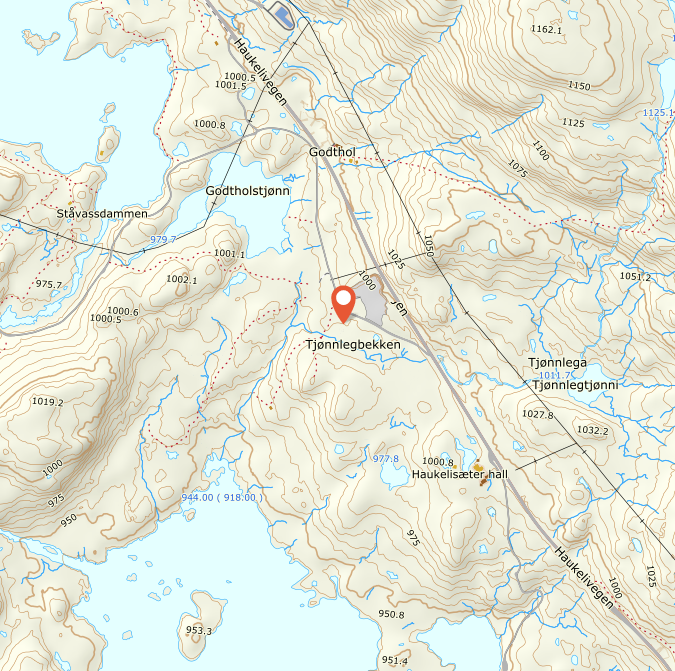
\includegraphics[width=\textwidth]{./fig_Norway/Haukeli_site}
% 		\caption{}\label{fig:site:kartverket}
% 	\end{subfigure}
% 	\caption{Model elevation map of Northern Europe (\protect\subref{fig:site:Norway}) and South Norway (\protect\subref{fig:site:Nzoom}). \subref{fig:site:Norway}  shows the model domain of MEPS.
% Elevation according to the shading. \protect\subref{fig:site:kartverket}: topographical map of the measurement site \citep{geonorge_dtm_2018}.} \label{fig:site}
% \end{figure}
%
% \begin{figure}[!t]
%   \begin{tabular}[t]{cc}
%     \begin{subfigure}[b]{0.5\columnwidth}
%       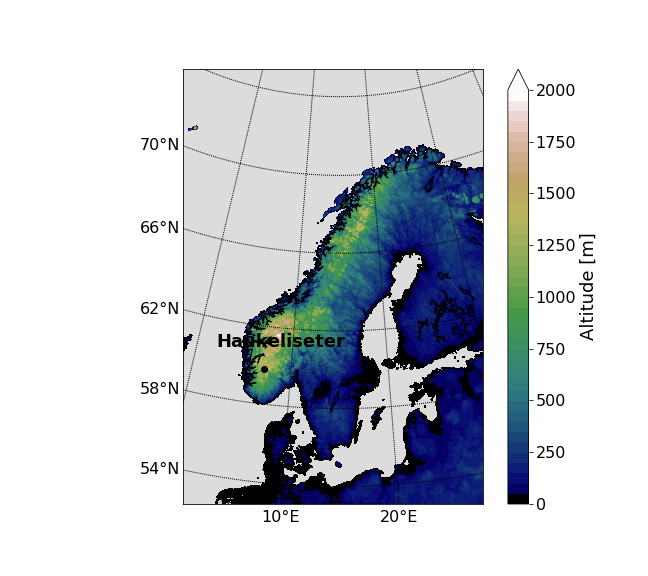
\includegraphics[trim={0cm 0cm 1.6cm 1.cm},clip,width=\textwidth]{./fig_Norway/Norway_elevation_MEPS}
%       \caption{}\label{fig:site:Norway}
%     \end{subfigure}
%     & 
%     \begin{tabular}[b]{c}
%       \begin{subfigure}[b]{0.5\columnwidth}
%         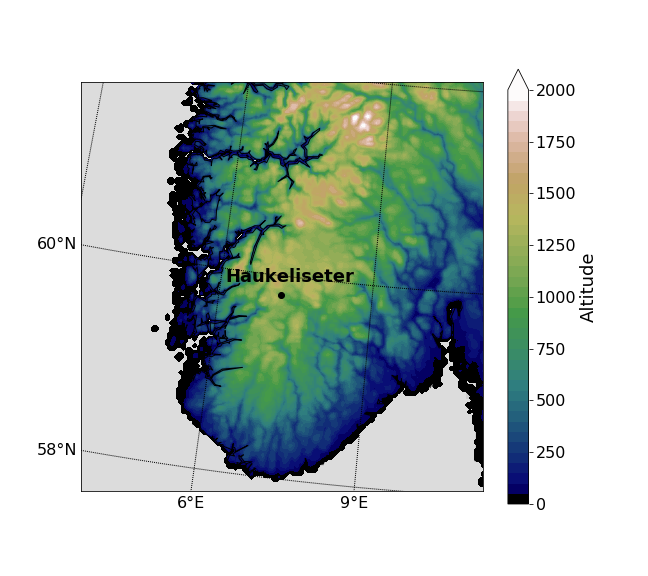
\includegraphics[trim={1.cm 2.2cm 1.8cm 2.4cm},clip,
%  		width=\textwidth]{./fig_Norway/South_Norway_MEPS}
%         \caption{}\label{fig:site:Nzoom}
%       \end{subfigure}\\
%       \begin{subfigure}[b]{0.52\columnwidth}
%         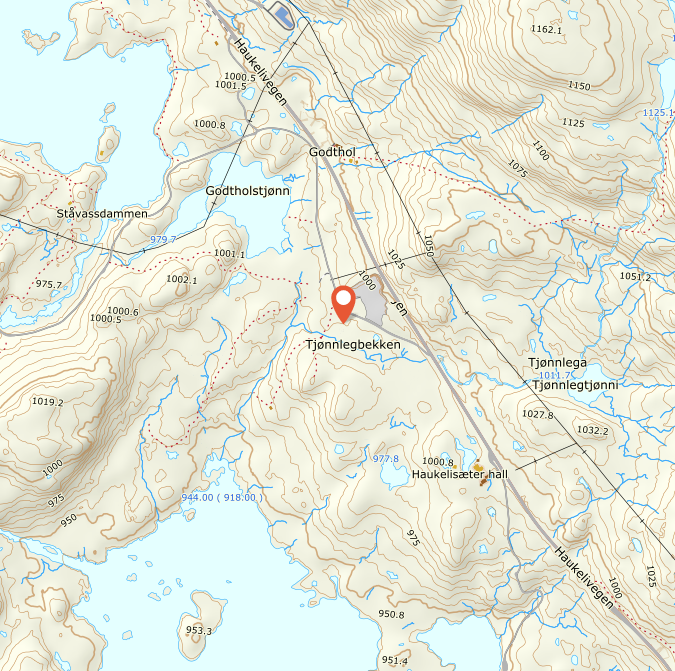
\includegraphics[trim={.3cm 2.2cm 1.8cm 2.4cm},clip,width=\textwidth]{./fig_Norway/Haukeli_site}
%         \caption{}\label{fig:site:kartverket}
%       \end{subfigure}
%     \end{tabular}
%   \end{tabular}
%   \caption{Model elevation map of Northern Europe (\protect\subref{fig:site:Norway}) and Southern Norway (\protect\subref{fig:site:Nzoom}), where the model domain of MEPS are presented in Lambert projection. The elevation corresponds to the legend of \protect\subref{fig:site:Nzoom}. A topographic map of the measurement site is shown in \protect\subref{fig:site:kartverket} \citep{kartverket_norgeskart_2018}.} \label{fig:site}
% \end{figure}
%%%%%%%%%%%%%%%%%%%%%%%%%%%%%%%%%%%%%%%%%%%%%%%%%%%%%%%%%%%%%%%%%%%%%%%%%%
Haukeliseter, shown in \Cref{fig:site} is a mountain plateau \SI{991}{\m} above sea level, located in the Norwegian county 'Telemark' (\ang{59.8}\,N, \ang{7.2}\,E, \Cref{fig:site}). The station measures precipitation, temperature, snow depth and wind. It has served as a measurement site for snow accumulation since the winter of 2010/2011 \citep{wolff_new_2010, wolff_measurements_2013, wolff_derivation_2015} and serves as WMO (World Meteorological Organization) station. \\
The study site is surrounded by mountain tops being \SIrange{100}{500}{\metre} higher than the flat area. As seen in \Cref{fig:site:kartverket} is Haukeliseter more open to the south and the south-west and the closest mountain top (situated to the NE) has an altitude of \SI{1162}{\metre a.s.l},  \citep{wolff_derivation_2015}. The mountains west to north exceed elevations of \SI{1600}{\metre}.
\\
A detailed setting of the measurement site is shown in \Cref{fig:inst_setting} with precipitation sensors perpendicular to the predominant wind. Additional measurements of other meteorological parameters such as temperature, wind, and pressure are used to get the large scale weather situation into a connection with the local measurements. The data is provided by \cite{eklima_norwegian_2016}, where the temperature is measured at double fence height. The hourly value of temperature is represented by the last minute value of the previous hour measurement. The \SI{10}{\metre} wind is measured by a ultrasonic wind sensor from Gill, mounted at the tower close to the double fence. The data represents the averaged \SI{10}{\minute} wind prior to the full hour.
%In a study by \cite{wolff_derivation_2015} the wind-induced under-catch of solid precipitation is determined. Dependent on the kind of precipitation the wind plays different roles in the amount of accumulation. For temperatures below \SI{-2}{\celsius} the wind speed influences the falling snow. Where less precipitation can be observed at higher wind speeds or more precipitation can be measured if too much is blown into the gauge. The catch ratio between the standard Geonor precipitation gauge and the Double Fence - Geonor shows, that only \SI{80}{\percent} of solid precipitation are observed at wind speeds of \SI{2}{\mPs} and only \SI{40}{\percent} at \SI{5}{\mPs}, \cite[Figure 5 in][]{wolff_derivation_2015}. The double fence gauge is more accurate than the single fence and is used as the reference gauge. A further description of the double fence is found in \Cref{sec:dofe}. 
%\textcolor{red}{Steve: Should make some reference here to the vertical profile of observations needed to evaluate MEPS.  Me: What exactly does he mean?}. 
%Nevertheless, this shows the need of a combination of ground based observations together with an optimal estimation retrieval to verify the accuracy of MEPS. \cite{wolff_derivation_2015} introduced an adjustment function for the Geonor double fence, so that different precipitation under certain wind speeds are presented correctly and can be used as confidential data. 
% \\ 
% \\
%
%
%
\section{Climate at Haukeliseter}\label{sec:dim:dec_obs}
The general climate at Haukeliseter can be defined with the updated K\"oppen-Geiger climate types presented in \cite{peel_updated_2007}. Figure 8 in \cite{peel_updated_2007} shows, that Haukeliseter may lay in a transition zone and can be categorized as  ET, a polar tundra climate type (hottest month temperature T$_{hot}\ge$ \SI{0}{\celsius}) or Dfc, a cold climate without dry season and cold summers. 
% %%% images December observation %%%%%%%%%%%%%%%%%%%%%%%%%%%%%%%%%%%%%
% % !TeX spellcheck = en_GB
\begin{figure}[!b]
	\centering
	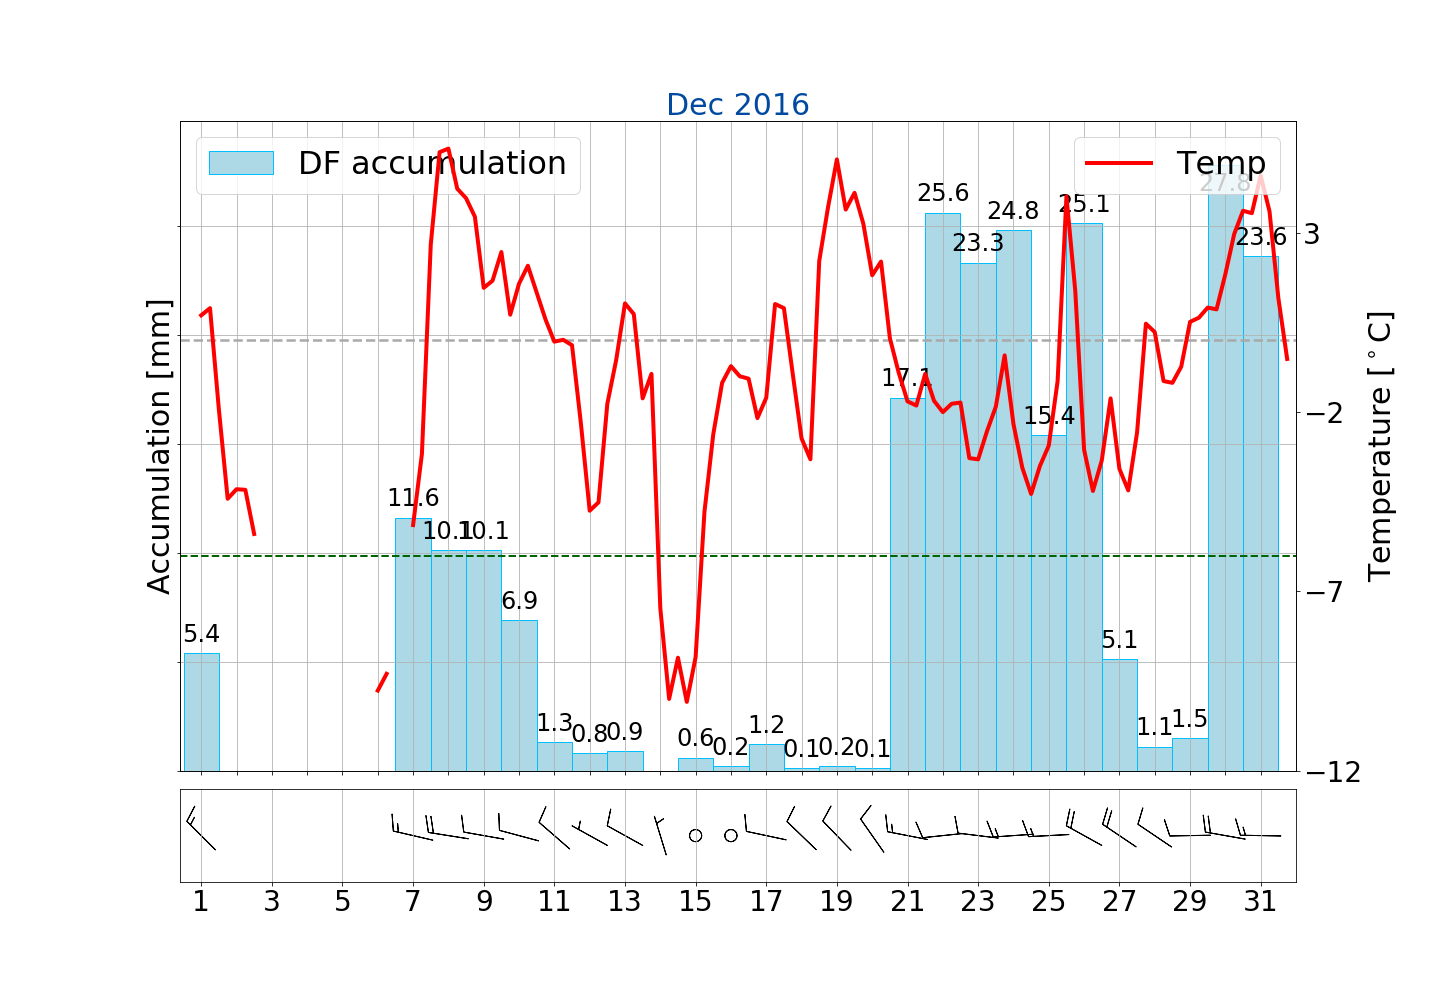
\includegraphics[trim={4.cm 3.3cm 1.5cm 3.cm},clip,
	width=0.65\textwidth]{./fig_weathermast/T_P_U_201612}
	\caption{Observations at Haukeliseter weather mast during December 2016. 
    The daily accumulation is presented in light blue [\SI{}{\mm}]; the six hour mean temperature in red, [\SI{}{\celsius}], and daily maximum \SI{10}{\metre} wind as barbs [\SI{}{\mPs}]. Gray dashed line indicates the freezing temperature. The freezing temperature is indicated by the green dashed line and the monthly normal value (\SI{-6.0}{\celsius}) by the green \citep{eklima_norwegian_2016}. Note, no data was available from \num{2} to \SI{6}{\dec}.} \label{fig:DecObs}
\end{figure}
% %%%%%%%%%%%%%%%%%%%%%%%%%%%%%%%%%%%%%%%%%%%%%%%%%%%%%%%%%%%%%%%%%%%%%%%%%%
Haukeliseter presents a typical Norwegian climate condition. At the measurement site, frequent snow events combined with high wind speeds are observed during a six to seven month winter period. In addition, a snow amount of about \SIrange{2}{3}{\m} can be expected, where \SI{50}{\percent} of the yearly precipitation is solid in the form of snow, graupel or mixed-phase precipitation \citep{wolff_new_2010, wolff_measurements_2013, wolff_derivation_2015}. \\
The mean wind direction (\Cref{fig:inst_setting}) for solid precipitation is from the west/east with maximum wind speeds above \SI{15}{\mPs}, observed during a 10 year winter period at a nearby station \citep{wolff_new_2010, wolff_derivation_2015}. 
%%% images December observation %%%%%%%%%%%%%%%%%%%%%%%%%%%%%%%%%%%%%
% !TeX spellcheck = en_GB
\begin{figure}[!b]
	\centering
	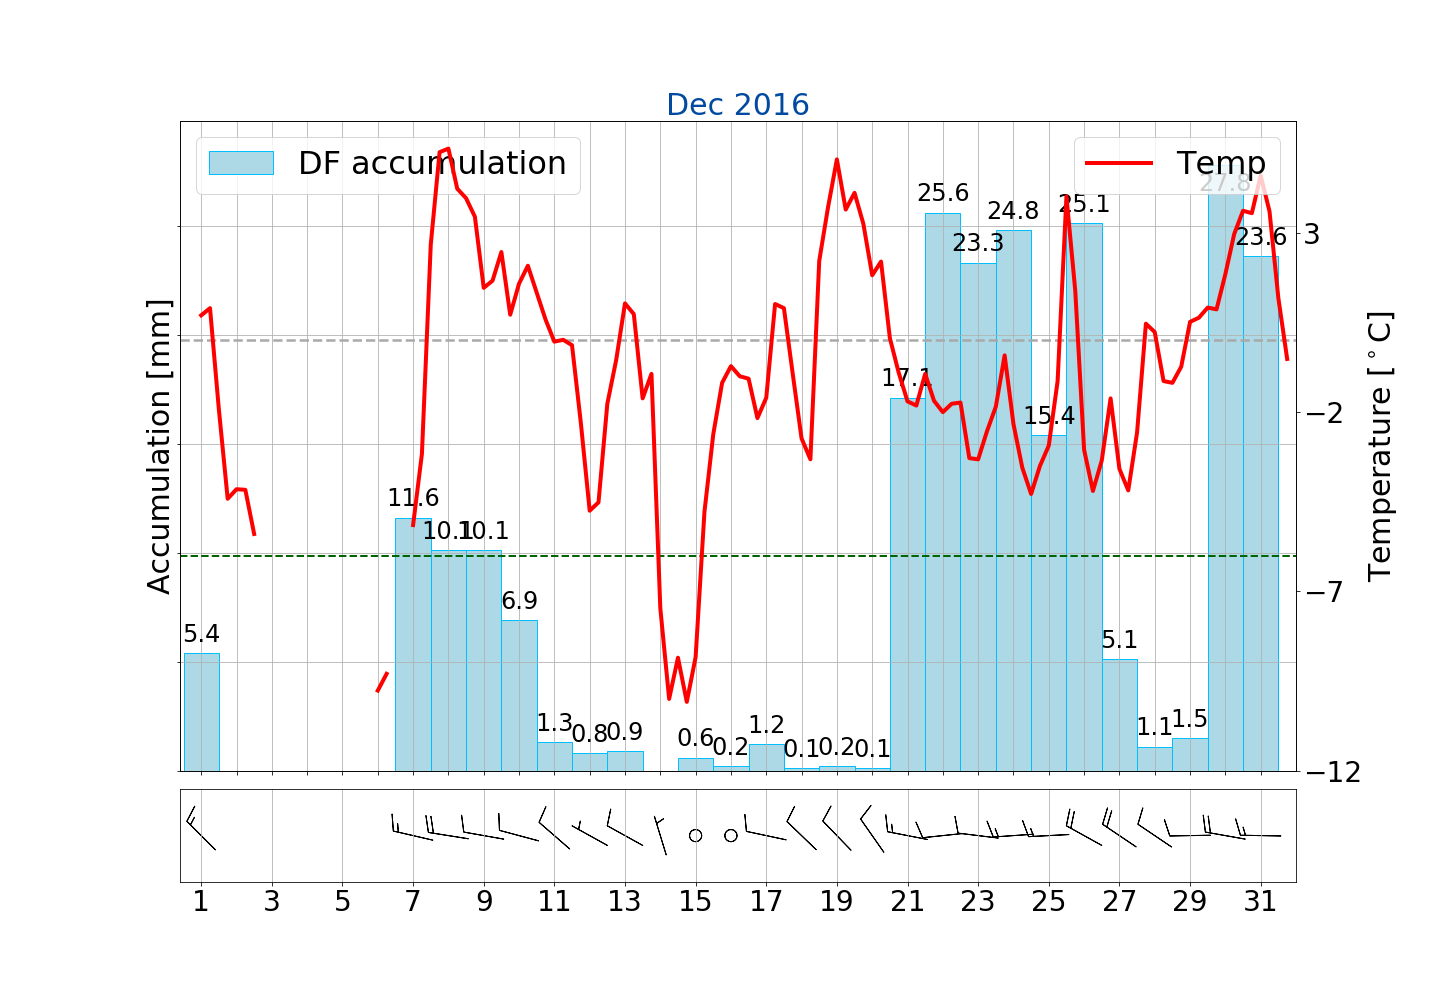
\includegraphics[trim={4.cm 3.3cm 1.5cm 3.cm},clip,
	width=0.65\textwidth]{./fig_weathermast/T_P_U_201612}
	\caption{Observations at Haukeliseter weather mast during December 2016. 
    The daily accumulation is presented in light blue [\SI{}{\mm}]; the six hour mean temperature in red, [\SI{}{\celsius}], and daily maximum \SI{10}{\metre} wind as barbs [\SI{}{\mPs}]. Gray dashed line indicates the freezing temperature. The freezing temperature is indicated by the green dashed line and the monthly normal value (\SI{-6.0}{\celsius}) by the green \citep{eklima_norwegian_2016}. Note, no data was available from \num{2} to \SI{6}{\dec}.} \label{fig:DecObs}
\end{figure}
%%%%%%%%%%%%%%%%%%%%%%%%%%%%%%%%%%%%%%%%%%%%%%%%%%%%%%%%%%%%%%%%%%%%%%%%%%
In \Cref{fig:DecObs}, the green dashed line, represents the average December temperature of \SI{-6}{\celsius} (30-yr period \numrange{1961}{1990}, value taken from \cite{eklima_norwegian_2016}).
% mean temperature in Dec was -1.1°C, climate = -6 --> dT = 4.9°C
December 2016 was warmer with an anomaly of +\SI{4.9}{\kelvin} above the climate mean. 
% total precipitation in Dec is 239.9mm, climate = 85mm --> dRR = 154.9
In 2016, the precipitation was \SI{200}{\percent} more than the climate mean during December. This difference could be associated with the new installation of the double fence - Genor gauge at Haukeliseter. In \cite{wolff_derivation_2015}, Figure 5 shows that single fence precipitation gauges underestimate the amount of precipitation about \SI{80}{\percent} during high wind speed events. Since the Double Fence construction was not in use before 2010/2011, this might have led to an observation of too little precipitation at Haukeliseter during winter and followed an incorrect climate statistic.
% total precipitation during 21.-27.12. is 136.4 mm, total is 239.9mm --> 56.9%
The precipitation observed in the time period \SIrange{21}{27}{\dec} where \SI{56.9}{\percent} of the total accumulation in December 2016. Furthermore, a maximum wind of \SI{22.3}{\mPs} was observed in this period, which can be associated to a slight storm, which is further described in \Cref{sec:loc_obs} and \Cref{tab:wind}.